\documentclass[10pt,a4paper]{article}
\usepackage[utf8]{inputenc}
\usepackage[italian]{babel}

\usepackage{amsmath}
\usepackage{mathtools}
\usepackage{amsfonts}
\usepackage{amssymb}
\usepackage{amsmath}
\usepackage{siunitx}
\usepackage{physics}

\mathtoolsset{showonlyrefs,showmanualtags}

\usepackage{graphicx}
\usepackage{subfig}
\usepackage{wrapfig}
\usepackage{sidecap}
\usepackage{booktabs}
\usepackage{hyperref}

\newtheorem{theorem}{Theorem}[section]
\newtheorem{corollary}{Corollary}[theorem]
\newtheorem{lemma}[theorem]{Lemma}

%%% BackEnd Bibliografico
%\usepackage{textcomp}
%\usepackage[autostyle]{csquotes}
%\usepackage[
%        backend=biber,
%        %bibstyle=numeric,
%        %sorting=ynt
%    ]{biblatex}
%\addbibresource{bibliografia.bib}
%\nocite{*}
%%%

%%%%%% TESTO EFFETTIVO

\title{Relazione Modelli e Metodi Numerici per la Fisica}
\author{Carlo Emilio Montanari}

\begin{document}

\maketitle

\tableofcontents

\newpage

%\begin{abstract}
%Nel presente elaborato si vuole analizzare nel dettaglio lo schema implicito di integrazione di Crank-Nicolson applicato ad una equazione generica di Fokker-Planck (diffusione con termine avvettivo). Nella prima parte si presenta lo schema, comparandolo al metodo di integrazione esplicito forward di Eulero, e si eseguono analisi standard di stabilità e convergenza prima nel contesto di una equazione di diffusione semplice e di una equazione di Fokker-Planck. % Nella seconda parte si analizzano le complicazioni computazionali che derivano nell'ampliamento dello schema a più dimensioni e si osservano possibili schemi alternativi più efficaci (Alternating Direction Implicit integration).
%\end{abstract}

\section{Equazione del calore e metodo esplicito}

Consideriamo l'equazione del calore nella sua forma più semplice su di un intervallo $x \in [0,1]$, con condizioni al contorno e condizioni iniziali date. Poniamo quindi:
\begin{equation}
	\pdv{u}{t} = \pdv[2]{u}{x} \quad\quad 0<x<1,\,t>0
	\label{eq:equazione_calore}
\end{equation}
con condizioni iniziali ed al contorno
\begin{align}
	u(x,t=0)=u_0(x) &\quad\quad 0\leq x\leq 1;\\
	u(0,t)=g_0(t),\, u(1,t)=g_1(t) &\quad\quad t\geq 0.
\end{align}
Dove abbiamo che $u_0(0) = g_0(0)$ e $u_0(1) = g_1(0)$ in modo da avere una soluzione continua.

Analizziamo ora come possiamo integrarla numericamente tramite metodo esplicito semplice. Come notazione considereremo lo spazio ed il tempo discretizzati nei seguenti termini:
\begin{align}
	x_m = mh, \quad m = 0,1,\dots,M, \quad (h=\frac{1}{M});\\
	t_n = nk, \quad n = 0,1,\dots,N, \quad (k=\frac{T_{\text{max}}}{N});
\end{align}
dove $T_{\text{max}}$ è il tempo fino al quale eseguiamo l'integrazione numerica.

\subsection{Integrazione con metodo esplicito}

Consideriamo le approssimazioni dei differenziali più semplici per rimpiazzare le derivate nell'equazione del calore:
\begin{align}
	\pdv{u}{t} &\to \frac{u_m^{n+1} - u_m^n}{k} + O(k),\\
	\pdv[2]{u}{x} &\to \frac{u_{m+1}^n-2u_m^n + u_{m-1}^n}{h^2} + O(h^2).
\end{align}
e, sostituendo tutto questo in \eqref{eq:equazione_calore}, otteniamo il metodo esplicito semplice:
\begin{equation}
	\frac{u_m^{n+1} - u_m^n}{k} = \frac{u_{m+1}^n-2u_m^n + u_{m-1}^n}{h^2} + O(k + h^2) 
	\label{eq:schema_esplicito}
\end{equation}
o, in forma più semplice,
\begin{equation}
	u_m^{n+1} = ru_{m+1}^n + (1-2r)u_m^n + ru_{m-1}^n,
	\label{eq:schema_esplicito_completo}
\end{equation}
con $r = k/h^2$.

\subsection{Analisi di stabilità}

Dall'equazione \eqref{eq:schema_esplicito} è evidente che lo schema considerato risulta consistente, nel senso che la differenza finita si avvicina alla soluzione vera dell'equazione differenziale mano a mano che le dimensioni degli step temporali e spaziali tende a zero. In altre parole, abbiamo che l'errore di troncamento $\tau$ soddisfa la condizione $\lim_{k,h\to 0}\tau = 0$.

Tuttavia, per poter affermare che il metodo numerico converga effettivamente alla soluzione analitica dell'equazione differenziale, dobbiamo anche assicurarci che lo schema sia anche stabile, dove per stabilità si intende che gli errori numerici fatti in uno step di calcolo non crescono significativamente negli step successivi.

Studiamo ora la stabilità di questo schema esplicito con due metodi diversi: analisi di stabilità della matrice e analisi di von Neumann.

\subsubsection{Analisi di stabilità della matrice}

Scriviamo l'equazione \eqref{eq:schema_esplicito_completo} in forma matriciale:
\begin{equation}
	\mqty*(u_1^{n+1}\\u_2^{n+1}\\ \cdot \\ \cdot \\ u_{M-1}^{n+1}) = \mqty*(1-2r & r & 0 & \cdot & \cdot & 0 \\ r & 1-2r & r & 0 & \cdot & 0 \\ \cdot & \cdot & \cdot & \cdot & \cdot & \cdot \\ 0 & \cdot & 0 & r & 1-2r & r \\ 0 & \cdot & \cdot & 0 & r & 1 - 2r) \mqty*(u_1^{n}\\u_2^{n}\\ \cdot \\ \cdot \\ u_{M-1}^{n})
\end{equation}
che equivale a scrivere
\begin{equation}
	\vb{u}^{n+1} = A \vb{u}^n.
\end{equation}
Questo schema converge alla soluzione solo se tutti gli autovalori di $A$ non hanno modulo superiore ad $1$. Se invece uno degli autovalori risultasse superiore ad $1$ (per esempio, $\lambda_1 > 1$), allora si avrebbe inevitabilmente che $\norm{u^n} = \norm{A^n u^0}$ avrà una crescita proporzionale a $\lambda_1^n$. È necessario quindi conoscere gli autovalori della matrice $A$ per poter regolare valori limite di conseguenza. Essendo $A$ una matrice in forma tridiagonale, vale il seguente lemma:

\begin{lemma}
	\label{lem:tridiagonale}
	Sia $B$ una matrice $N \times N$ una matrice in forma tridiagonale
	\begin{equation}
		\mqty*(b & c & 0 & \cdot & \cdot & 0 \\ a & b & c & 0 & \cdot & 0 \\ \cdot & \cdot & \cdot & \cdot & \cdot & \cdot \\ 0 & \cdot & 0 & a & b & c \\ 0 & \cdot & \cdot & 0 & a & b).
	\end{equation}
	Gli autovalori ed i corrispettivi autovettori della matrice $B$ sono:
	\begin{equation}
		\lambda_j = b+2\sqrt{ac} \cos{\frac{\pi j}{N+1}}
	\end{equation}
	\begin{equation}
		\vb{v}_j = \mqty*(\left(\frac{a}{c}\right)^{1/2}\sin{\frac{1\cdot\pi j}{N+1}} \\ \left(\frac{a}{c}\right)^{2/2}\sin{\frac{2\cdot\pi j}{N+1}} \\ \cdot \\ \cdot \\ \left(\frac{a}{c}\right)^{N/2}\sin{\frac{N\cdot\pi j}{N+1}})
	\end{equation}
	con $j = 1,\ldots, N$.
\end{lemma}

Da questo lemma, ricaviamo subito che gli autovalori della matrice $A$ sono
\begin{equation}
	\lambda_j = 1-2r+2r\cos{\frac{\pi j}{M}}, \quad\quad j=1,\ldots,M-1,
\end{equation}
da cui consegue che
\begin{align}
	\lambda_{\text{min}} &= \lambda_{M-1} = 1-2r+2r\cos{\frac{\pi (M-1)}{M}},\\
	\lambda_{\text{max}} &= \lambda_1 = 1-2r+2r\cos{\frac{\pi}{M}}.
\end{align}
Se $\pi / M \ll 1$ (i.e. la discretizzazione dell'intervallo $[0,1]$ è sufficientemente piccola), è possibile approssimare i due autovalori nella forma
\begin{align}
	\lambda_{\text{min}} &\approx 1-4r+r\left(\frac{\pi}{M}\right)^2,\\
	\lambda_{\text{max}} &\approx 1 -r\left(\frac{\pi}{M}\right)^2,
\end{align}
dove si è fatto uso dell'espansione $\cos\alpha \approx 1- \frac{1}{2}\alpha^2$ per $\alpha \ll 1$. A questo punto per far rispettare la condizione di convergenza imposta prima
\begin{equation}
	-1 \leq \lambda_j \leq 1, \quad\quad j = 1,\ldots, M-1,
\end{equation}
porta a dover avere
\begin{align}
	\lambda_{\text{min}} &\approx 1-4r+r\left(\frac{\pi}{M}\right)^2 \geq -1,\\
	\lambda_{\text{max}} &\approx 1 -r\left(\frac{\pi}{M}\right)^2 \leq 1.
\end{align}
La seconda equazione è sempre rispettata in quanto $r = k/h^2 > 0$. La prima equazione comporta invece
\begin{equation}
	r \leq \frac{2}{4-\left(\frac{\pi}{M}\right)^2} = \frac{2}{4-(\pi h)^2}\approx \frac{1}{2},
\end{equation}
che, considerando sempre la definizione di $r$, equivale a scrivere
\begin{equation}
	k \leq \frac{1}{2} h^2.
	\label{eq:stabilita_esplicito}
\end{equation}
Se questa condizione viene rispettata, si ha che tutti gli errori di round-off eventualmente decadranno, e che quindi questo schema esplicito è numericamente stabile.

\subsubsection{Analisi di stabilità di von Neumann}

Questo caso in analisi risulta estremamente favorevole in quanto la matrice $A$ si presenta in una forma particolarmente semplice da analizzare. Tuttavia, nella maggior parte dei casi, risulta impossibile una analisi degli autovalori come quella fatta sopra ed è pertanto necessario analizzare la stabilità senza fare uso degli autovalori stessi.

Osserviamo quindi che, essendo l'equazione del calore \eqref{eq:equazione_calore} e la sua corrispondente versione discretizzata \eqref{eq:schema_esplicito_completo} lineari, anche l'errore computazionale soddisferà le equazioni al pari della soluzione stessa. Se definiamo l'errore al punto di calcolo $(mh, nk)$ come $\epsilon_m^n$, avremo che questo soddisferà l'equazione:
\begin{equation}
	\epsilon_m^{n+1} = r \epsilon_{m+1}^n + (1-2r)\epsilon_m^n + r \epsilon_{m-1}^n.
	\label{eq:errore_schema_esplicito}
\end{equation}
In ogni step temporale, l'errore può essere espanso in forma di serie di Fourier:
\begin{equation}
	\epsilon_m^n = \sum_l c_l(n)\exp(i\beta_l x_m)
\end{equation}
dove il range di valori di $\beta_l$ verrà specificato successivamente.

Essendo l'equazione \eqref{eq:errore_schema_esplicito} lineare, possiamo sostituire ogni $\epsilon$ con la sua corrispettiva espansione. Nel farlo indichiamo anche
\begin{equation}
	c_l(n) = \rho^n
\end{equation}
dove $\rho$ è il valore numerico da determinare. A questo punto, sostituendo $\epsilon_m^n = \rho^n \exp(i\beta mh)$ in \eqref{eq:errore_schema_esplicito}, si ottiene (si considera un solo termine dell'espansione di Fourier):
\begin{equation}
	\rho^{n+1} e^{i\beta mh} = r\rho^n e^{i\beta(m+1)h}+(1-2r)\rho^n e^{i\beta mh} + r\rho^n e^{i\beta (m-1)h}.
\end{equation}
Dove in questo caso l'indice in alto per $\rho$ indica un elevamento a potenza (a differenza dell'indice in alto per $\epsilon$ che sta ad indicare lo step temporale di calcolo). Semplificando questa equazione si ha
\begin{equation}
	\rho = r e^{i\beta h}+ (1-2r) + re^{-i\beta h} = 1 - 2r + 2r \cos(\beta h).
\end{equation}
Volendo quindi imporre la condizione $\abs{\rho}\leq 1$, che ci garantisce che l'errore numerico non crescerà, si ottiene:
\begin{equation}
	-1 \leq 1 - 2r + 2r\cos(\beta h) \leq 1.
	\label{eq:fourier_error}
\end{equation}

Per capire quindi come questa condizione si riflette su $r$, dobbiamo stabilire quali valori $\beta$ può assumere. In un approccio semplificato, assumiamo che il coseno in equazione \eqref{eq:fourier_error} possa assumere l'intero range di valori possibili:
\begin{equation}
	-1 \leq \cos(\beta h) \leq 1 \quad\Rightarrow\quad 0 \leq \beta h \leq \pi.
\end{equation}
Sfruttando quindi la formula, valida per ogni $\alpha$:
\begin{equation}
	1-\cos{\alpha} = 2 \sin^2\left(\frac{\alpha}{2}\right)
\end{equation}
si può riscrivere \eqref{eq:fourier_error} nella forma
\begin{equation}
	-1 \leq 1 - 4r \sin^2\left(\frac{\beta h}{2}\right) \leq 1. 
\end{equation}
La disuguaglianza a destra vale sempre, mentre quella a sinistra implica:
\begin{equation}
	r \sin^2\left(\frac{\beta h}{2}\right) \leq 1/2.
\end{equation}
Di conseguenza, per garantire la stabilità del metodo, questa disuguaglianza deve valere per ogni valore di $\beta h$. In particolare, è sufficiente che valga per il `caso peggiore' che porta ad avere il valore massimo di $\sin^2(\beta h/2)$. Questo valore corrisponde ad $1$ e lo si ha nel caso in cui $\beta h = \pi$. In tal caso, la condizione di stabilità è
\begin{equation}
	r \cdot 1 \leq \frac{1}{2},
\end{equation}
che è una condizione di stabilità semplificata rispetto alla condizione di stabilità ottenuta con il metodo di analisi di stabilità della matrice, che è invece la condizione \textit{esatta} di stabilità tenendo conto delle condizioni di contorno. Qualora avessimo voluto ottenere risultati altrettanto affinati con questo metodo sarebbe stato necessario analizzare come le condizioni al contorno interferiscono con i modi dell'espansione di Fourier.

\subsection{Risultati numerici}

Considerando come problema di prova l'equazione del calore sempre nell'intervallo $x\in[0,1]$ con le seguenti condizioni iniziali ed al contorno $(D=1)$:
\begin{align}
	\pdv{u}{t} &= D \pdv[2]{u}{x}, \quad\quad 0\leq x \leq 1\\
	u(x,0) &= \sin(\pi x)\\
	u(0,t) &= 0\\
	u(1,t) &= 0
\end{align}
Abbiamo che la soluzione analitica è (si veda Appendice \ref{app:soluzione_esatta}):
\begin{equation}
	u(x,t) = \sin(\pi x)\exp(- D \pi^2 t).
\end{equation}

\subsubsection{Stabilità}

Abbiamo osservato prima che il metodo, per dati valori di $r$, può presentare situazioni di instabilità, si può osservare infatti dalla figura \ref{fig:stabilita_esplicito} come l'integrazione numerica comincia a presentare errori drammatici già dopo pochi step numerici.

\subsubsection{Verifica delle stime degli errori di troncamento}
\label{subsec:tronc_exp}
Definiamo come misura dell'errore di troncamento
\begin{equation}
	\epsilon_m = \norm{u_i^m - u(x_i,t_m)}_2
\end{equation}
dove $u_i^m$ è il valore ottenuto con lo schema numerico e $u(x_i,t_m)$ la corrispondente soluzione analitica.

Vogliamo analizzare se e come effettivamente l'errore tende a zero andando a modificare i valori di differenze finite di spazio e di tempo. Si considera sempre un valore di $D = 1$ed uno spazio $x \in [0,1]$. Si va a considerare l'evoluzione di $\epsilon$ nell'intervallo temporale $t=[0,0.5]$ per diversi valori di $k = \Delta t$ e $h = \Delta x$. Andando poi a graficare il valore massimo di errore registrato ad ogni diversa esecuzione (figura \ref{fig:explicito}), si comincia già ad osservare un primo andamento confermante l'errore di troncamento $O(h+k^2)$.

\begin{figure}
	\centering
	\subfloat[][Andamento lineare.]{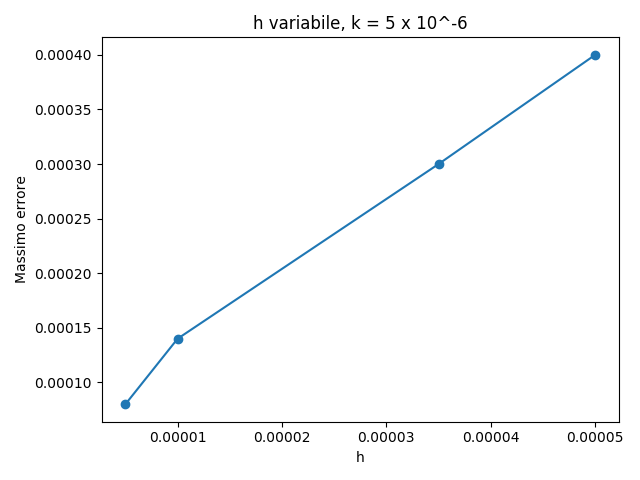
\includegraphics[width=0.4\textwidth]{img/explicit_h.png}}\quad
	\subfloat[][Andamento quadratico.]{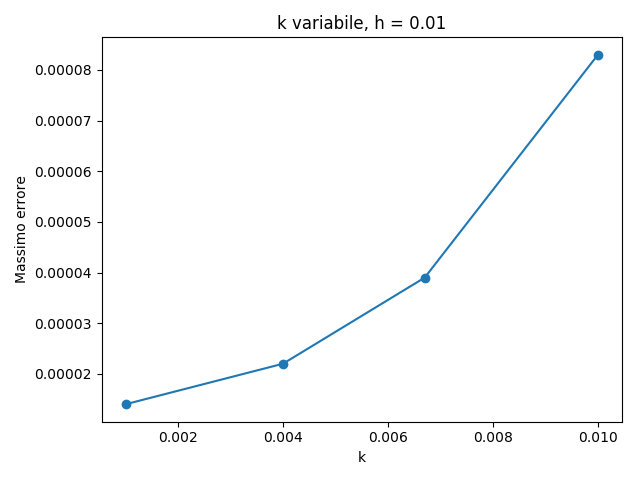
\includegraphics[width=0.4\textwidth]{img/explicit_k.png}}
	\caption{Valori massimi di errore per variazioni di $h$ e $k$.}
	\label{fig:explicito}
\end{figure}

%%%%%%%%%%%%%%%%%%%%%%%%%%%%%%%%%%%%%%%%%%%%%%%%%%%%
%%%%%%%%%%%%%%%%%%%%%%%%%%%%%%%%%%%%%%%%%%%%%%%%%%%%
%%%%%%%%%%%%%%%%%%%%%%%%%%%%%%%%%%%%%%%%%%%%%%%%%%%%
%%%%%%%%%%%%%%%%%%%%%%%%%%%%%%%%%%%%%%%%%%%%%%%%%%%%
%%%%%%%%%%%%%%%%%%%%%%%%%%%%%%%%%%%%%%%%%%%%%%%%%%%%
%%%%%%%%%%%%%%%%%%%%%%%%%%%%%%%%%%%%%%%%%%%%%%%%%%%%

\section{Equazione del calore e metodo di Crank-Nicolson}
\label{sec:2}

Data una equazione a derivate parziali nella forma
\begin{equation}
	\pdv{u}{t} = F\left(u,x,t,\pdv{u}{x},\pdv[2]{u}{x}\right)
\end{equation}
il metodo di Crank-Nicolson si presenta come una combinazione del metodo Forward di Eulero (visto nella sezione precedente) e del metodo Backward di Eulero, tenendo conto del fatto che non si sta lavorando con una semplice media tra i due metodi in quanto vi sono dipendenze implicite tra le varie soluzioni:
\begin{align}
	\frac{u_m^{n+1}-u_m^n}{k} &= F_m^n\left(u,x,t,\pdv{u}{x},\pdv[2]{u}{x}\right) \quad &\text{(Forward)}\\
	\frac{u_m^{n+1}-u_m^n}{k} &= F_m^{n+1}\left(u,x,t,\pdv{u}{x},\pdv[2]{u}{x}\right) \quad &\text{(Backward)}\\
	\frac{u_m^{n+1}-u_m^n}{k} &= \frac{1}{2}\left[F_m^n\left(u,x,t,\pdv{u}{x},\pdv[2]{u}{x}\right) + F_m^{n+1}\left(u,x,t,\pdv{u}{x},\pdv[2]{u}{x}\right)\right] \label{eq:crank-nicolson}
\end{align}
Essendo \eqref{eq:crank-nicolson} un metodo implicito, per ottenere il valore 'successivo` di $u$ rispetto al tempo è necessario risolvere un sistema di equazioni.

Nel contesto dell'equazione \eqref{eq:equazione_calore}, $F_m^n$ assume la forma
\begin{equation}
	F_m^n(u) = \frac{u_{m+1}^n - 2u_m^n + u_{m-1}^n}{h^2}
\end{equation}
ergo, lo schema intero ha forma
\begin{equation}
	\frac{u_m^{n+1}-u_m^n}{k} = \frac{1}{2} \left[\frac{u_{m+1}^n - 2u_m^n + u_{m-1}^n}{h^2} + \frac{u_{m+1}^{n+1} - 2u_m^{n+1} + u_{m-1}^{n+1}}{h^2}  \right]
\end{equation}
o, definendo la seguente notazione
\begin{align}
	\frac{1}{h^2}\delta_x^2 u_m &\equiv \frac{u_{m+1}-2u_m+u_{m-1}}{h^2}\\
	\frac{1}{k}\delta_t u^n &\equiv \frac{u^{n+1}-u^n}{k}
\end{align}
abbiamo la forma semplificata
\begin{equation}
	\frac{1}{k} \delta_t u_m^n = \frac{1}{2h^2}[\delta_x^2 u_m^n + \delta_x^2 u_m^{n+1}],
	\label{eq:crank_semplificato}
\end{equation}
che può quindi essere riscritta nella forma
\begin{equation}
	\left(1-\frac{r}{2}\delta_x^2\right) u_m^{n+1} = \left(1+\frac{r}{2} \delta_x^2\right) u_m^n, \quad\quad m = 1,\ldots,M-1,
	\label{eq:schema_crank-nicolson}
\end{equation}
dove $r = k/h^2$.

Lo schema \eqref{eq:schema_crank-nicolson} può essere quindi scritto in forma vettoriale
\begin{equation}
	\left(I - \frac{r}{2} A\right)\vb{u}^{n+1} = \left(I + \frac{r}{2} A\right)\vb{u}^n + \vb{b},
\end{equation}
dove $I$ è la matrice identità e
\begin{align}
	A &= \mqty*(-2 & 1 & 0 & \cdot & \cdot & 0 \\ 1 & -2 & 1 & 0 & \cdot & 0 \\ \cdot & \cdot & \cdot & \cdot & \cdot & \cdot \\ 0 & \cdot & 0 & 1 & -2 & 1 \\ 0 & \cdot & \cdot & 0 & 1 & -2);\label{eq:A_calore_CN}\\
	\vb{b} &= \frac{r}{2}\mqty*(u_0^n + u_0^{n+1} \\ 0 \\ \cdot \\ 0 \\ u_M^n + u_M^{n+1}) \equiv \frac{r}{2}\mqty*(g_0(t_n) + g_0(t_{n+1}) \\ 0 \\ \cdot \\ 0 \\ g_M(t_n) + g_M(t_{n+1})).
\end{align}
Si ha quindi da risolvere per ogni iterazione un sistema lineare tridiagonale, per farlo esistono algoritmi di complessità $O(M)$ che permettono di avere tempi di calcolo ragionevoli.

\subsection{Errore di troncamento nel metodo di Crank-Nicolson}
\label{sec:troncamento}

Osservando lo schema del metodo di Crank-Nicolson, si nota che questo è simmetrico rispetto al nodo virtuale $(mh, (n+ \frac{1}{2})k)$, questo rende pratico compiere una espansione in quel punto. Definiamo
\begin{equation}
	\bar{u} \equiv u\left(mh, (n + \frac{1}{2})k\right).
\end{equation}
A questo punto, eseguendo una espansione di Taylor su due variabili, otteniamo (per $\epsilon = -1,0,1$):
\begin{align}
	u_{m+\epsilon}^{n+1} = \bar{u}_m &+ \left( \frac{k}{2}\bar{u}_{m,t} + \epsilon h \bar{u}_{m,x} \right)\\
	&+ \frac{1}{2!}\left(\left(\frac{k}{2}\right)^2 \bar{u}_{m,tt} + 2 \frac{k}{2}\epsilon h \bar{u}_{m,xt}+(\epsilon h)^2 \bar{u}_{m,xx}\right)\\
	&+ \frac{1}{3!}\left(\left(\frac{k}{2}\right)^3 \bar{u}_{m,ttt} + 3\left(\frac{k}{2}\right)^2 \epsilon h \bar{u}_{m,xtt} + 3 \frac{k}{2}(\epsilon h)^2 \bar{u}_{m,xxt}+ (\epsilon h)^3 \bar{u}_{m,xx}\right)\\
	&+O(k^4+k^3h+k^2h^2+kh^3+h^4),
\end{align}
dove si indica con il secondo gruppo di indici in basso una derivazione per $x$ o per $t$ secondo la notazione $\bar{u}_{m,t} = \pdv{}{t}u_m|_{t=(n+\frac{1}{2})k}$.\\Similmente, abbiamo che
\begin{align}
	u_{m+\epsilon}^{n} = \bar{u}_m &+ \left( -\frac{k}{2}\bar{u}_{m,t} + \epsilon h \bar{u}_{m,x} \right)\\
	&+ \frac{1}{2!}\left(\left(-\frac{k}{2}\right)^2 \bar{u}_{m,tt} + 2 \left(-\frac{k}{2}\right)\epsilon h \bar{u}_{m,xt}+(\epsilon h)^2 \bar{u}_{m,xx}\right)\\
	&+ \frac{1}{3!}\left(\left(-\frac{k}{2}\right)^3 \bar{u}_{m,ttt} + 3\left(-\frac{k}{2}\right)^2 \epsilon h \bar{u}_{m,xtt} + 3 \left(-\frac{k}{2}\right)(\epsilon h)^2 \bar{u}_{m,xxt}+ (\epsilon h)^3 \bar{u}_{m,xx}\right)\\
	&+O(k^4+k^3h+k^2h^2+kh^3+h^4),
\end{align}
andando poi a sostituire con queste espressioni dentro l'equazione \eqref{eq:crank_semplificato} ponendo $\epsilon = 0$ e sfruttando le componenti dell'espansione fino all'ordine opportuno, si ottiene
\begin{equation}
	\frac{1}{k} \delta_t u_m^n = \bar{u}_{m,t} + O(k^2)
\end{equation}
e
\begin{equation}
	\frac{1}{2h^2}(\delta_x^2 u_m^n + \delta_x^2 u_m^{n+1}) = \bar{u}_{m,xx} + O(k^2 + h^2)
\end{equation}
che porta quindi a dire che
\begin{equation}
	\frac{1}{k} \delta_t u_m^n - \frac{1}{2h^2}(\delta_x^2 u_m^n + \delta_x^2 u_m^{n+1}) = \bar{u}_{m,t} - \bar{u}_{m,xx} + O(k^2, h^2),
\end{equation}
che sta a significare che l'errore di troncamento dello schema è al secondo ordine sia sullo spazio che sul tempo.

\subsection{Analisi di stabilità}

Per comprendere a pieno la natura e le proprietà dello schema di Crank-Nicolson, consideriamo la seguente generalizzazione dello schema implicito di Eulero:
\begin{equation}
	\vb{u}^{n+1} = \vb{u}^n + k((1-\theta)\vb{F}^{n} + \theta \vb{F}^{n+1})
\end{equation}
dove la costante $\theta$ assume valori reali nell'intervallo $[0,1]$, si denomina questa generalizzazione di metodi come $\theta$-famiglia di metodi. Nel contesto dell'equazione del calore \eqref{eq:equazione_calore} questa assume forma
\begin{equation}
	(I-r\theta A)\vb{u}^{n+1} = (I+r(1-\theta)A)\vb{u}^n + \vb{b}.
	\label{eq:theta_scheme}
\end{equation}
Andremo quindi ad analizzare direttamente la stabilità della $\theta$-famiglia, per poi considerare il caso specifico del metodo di Crank-Nicolson che corrisponde a $\theta = 1/2$.

\subsubsection{Analisi di stabilità della matrice}
\label{sec:stabilita_matrice}

L'equazione a derivate parziali che stiamo trattando in questo contesto è lineare, ergo sia la soluzione che l'errore in termini dello schema numerico soddisfano l'equazione differenziale con la stessa parte omogenea: in particolare, in questo caso, equazione \eqref{eq:theta_scheme} con $\vb{b}=0$. Di conseguenza, per stabilire la condizione di stabilità di questo schema consideriamo solo la parte omogenea, in quanto le componenti non omogenee (i.e., $\vb{b}$) non ne alterano le proprietà.

Cominciamo col porre lo schema in forma matriciale
\begin{equation}
	\vb{u}^{n+1} = \mathcal{M}\vb{u}^n
\end{equation}
abbiamo quindi il modulo degli autovalori di $\mathcal{M}$ da analizzare, per vedere se superano il valore di $1$. Possiamo avere una delle seguenti situazioni:
\begin{itemize}
	\item Se almeno uno degli autovalori $\lambda_j$ è tale che $\abs{\lambda_j}>1$ allora lo schema è instabile.
	\item Se si ha al massimo un autovalore tale che $\abs{\lambda_j}=1$, con tutti gli altri autovalori strettamente minori di $1$ in modulo, allora lo schema è stabile.
	\item Se si hanno più autovalori $\abs{\lambda_{j1}} = \ldots = \abs{\lambda_{jJ}} = 1$ con gli altri valori strettamente minori di $1$ in modulo si possono avere due situazioni diverse,
	\begin{enumerate}
	 	\item Tutti gli autovettori corrispondenti agli autovalori di modulo $1$ sono distinti, in tal caso lo schema è stabile.
	 	\item Se invece vi sono autovettori identici (o se si ha un autovalore doppio), allora lo schema è instabile, pur avendo un errore che cresce lentamente.
	\end{enumerate} 
\end{itemize}

Riscrivendo quindi equazione \eqref{eq:theta_scheme} con $\vb{b}$ posto a zero abbiamo
\begin{equation}
	\vb{u}^{n+1} = (I-r\theta A)^{-1}(I+r(1-\theta)A)\vb{u}^n.
\end{equation}
Sappiamo dall'algebra lineare che, date tre matrici $A, (aA+bI), (cA+dI)^{-1}$, queste hanno gli stessi autovettori con corrispettivi autovalori scrivibili rispettivamente nella forma $\theta, (a\theta + b), (c\theta +d)^{-1}$. Di conseguenza, detti $\lambda_j$ gli autovalori noti della matrice tridiagonale $A$, abbiamo che gli autovalori della matrice $\mathcal{M}$ in questo contesto possono essere scritti nella forma
\begin{equation}
	\frac{1+r(1-\theta)\lambda_{j}}{1-r\theta\lambda_j},
\end{equation}
dai conti precedenti sappiamo poi che
\begin{equation}
	\lambda_j = -4 \sin^2\left(\frac{\pi j}{2M}\right),\quad\quad j=1,\ldots,M.
\end{equation}
Ponendo quindi per comodità $\phi_j = \pi j/2M$, possiamo riscrivere la condizione di stabilità
\begin{equation}
	\abs{\frac{1+r(1-\theta)\lambda_{j}}{1-r\theta\lambda_j}}\leq 1, \quad\quad j=1,\ldots,M
\end{equation}
nella forma
\begin{equation}
	\abs{1-4r(1-\theta)\sin^2{\phi_j}}\leq\abs{1+4r\theta\sin^2{\phi_j}}
\end{equation}
ed essendo la parte dentro il modulo a destra della disuguaglianza sempre positiva, possiamo scrivere
\begin{equation}
	-(1-4r(1-\theta)\sin^2{\phi_j})\leq{1+4r\theta\sin^2{\phi_j}}\leq 1-4r(1-\theta)\sin^2{\phi_j}
\end{equation}
dove in questa disuguaglianza doppia la parte a destra è sempre soddisfatta per ogni $\phi_j$, mentre la parte a sinistra è soddisfatta quando
\begin{equation}
	4r(1-2\theta)\sin^2\phi_j \leq 2.
\end{equation}
Il `worst-case' per $r$ lo si ha quando $\sin^2 \phi_j = 1$, in questo caso si ha direttamente
\begin{equation}
  	(1-2\theta)r\leq\frac{1}{2}.
\end{equation}  
Si possono quindi distinguere 2 casi significativi
\begin{enumerate}
	\item Se $0\leq\theta < 1/2$, si ha che lo schema è stabile fintanto che vale la relazione
	\begin{equation}
	 	r\leq\frac{1}{2(1-2\theta)}.
	\end{equation}
	\item Se $1/2 \leq \theta \leq 1$, si ha che lo schema è \textbf{incondizionatamente stabile}, nel senso che qualsiasi valore di $r$ assicura la stabilità dello schema \eqref{eq:theta_scheme}.
\end{enumerate}

Essendo lo schema di Crank-Nicolson caratterizzato da $\theta = 1/2$, abbiamo che questo è incondizionatamente stabile, pertanto non sono necessarie particolari relazioni tra $k$ e $h$ per avere stabilità numerica. Questo è uno dei vantaggi principali nell'utilizzo di questo schema.

\subsection{Risultati numerici}
 
Si lavora con la stessa soluzione nota trattata in Appendice \ref{app:soluzione_esatta}.

\subsubsection{Stabilità}

Si può osservare da Figura multipla \ref{fig:stabilita_implicito} come diversi valori di $r$ non pregiudicano la stabilità dell'integrazione numerica.

\subsubsection{Troncamento}
\label{subsec:tronc_imp}

Eseguendo lo stesso ragionamento nel caso esplicito, si riportano i risultati in Figura \ref{fig:troncamento_implicito}.

\begin{figure}
	\centering
	\subfloat[][$h = 0.002,\quad k = 1\times10^{-2}$]{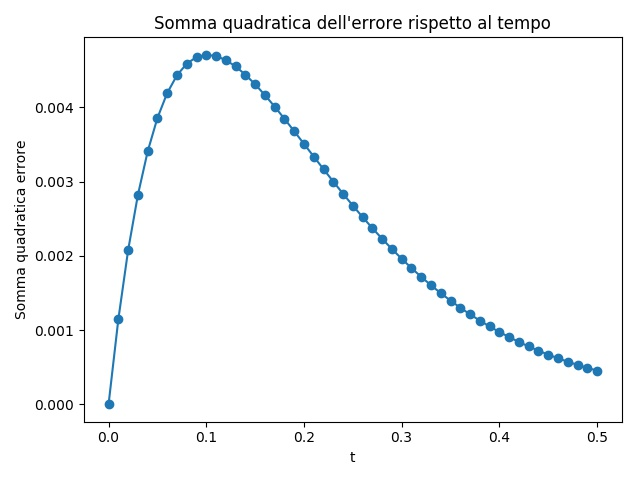
\includegraphics[width=0.4\textwidth]{img/het_cn_M501_N50.jpg}}
	\subfloat[][$h = 0.002,\quad k = 5\times10^{-3}$]{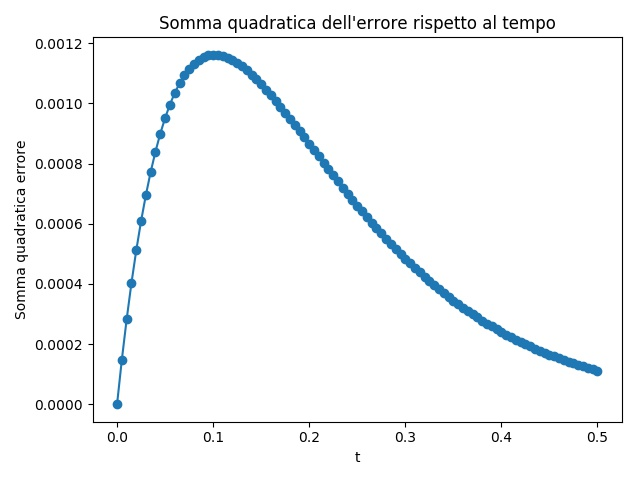
\includegraphics[width=0.4\textwidth]{img/het_cn_M501_N100.jpg}}\\
	\subfloat[][$h = 0.002,\quad k = 1\times10^{-3}$]{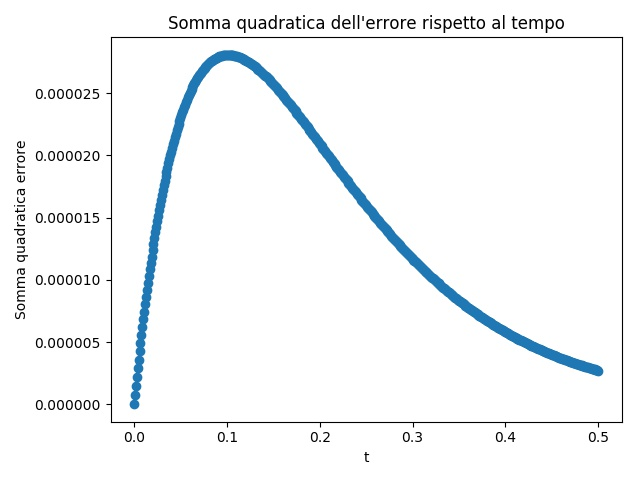
\includegraphics[width=0.4\textwidth]{img/het_cn_M501_N500.jpg}}
	\subfloat[][$h = 0.002,\quad k = 5\times10^{-4}$]{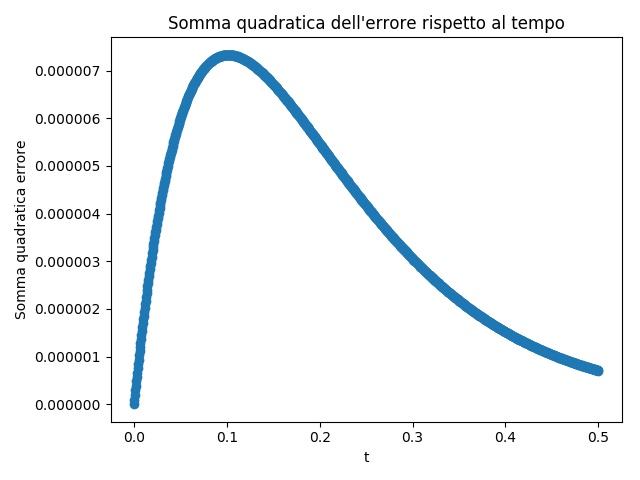
\includegraphics[width=0.4\textwidth]{img/het_cn_M501_N1000.jpg}}\\
	\subfloat[][$h = 0.1,\quad k = 5\times10^{-6}$]{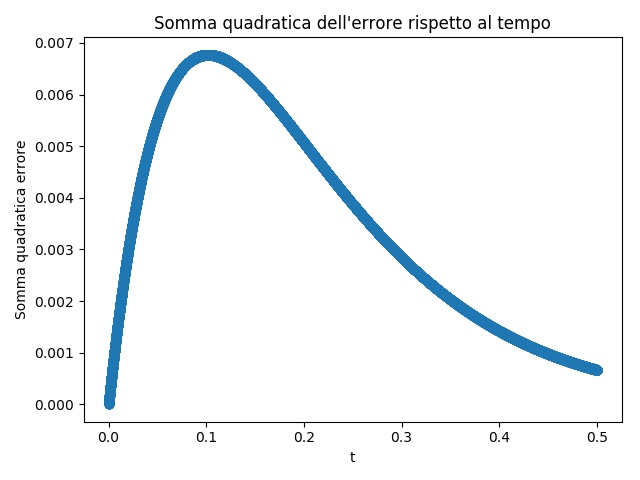
\includegraphics[width=0.4\textwidth]{img/het_cn_M11_N100000.jpg}}
	\subfloat[][$h = 0.05,\quad k = 5\times10^{-6}$]{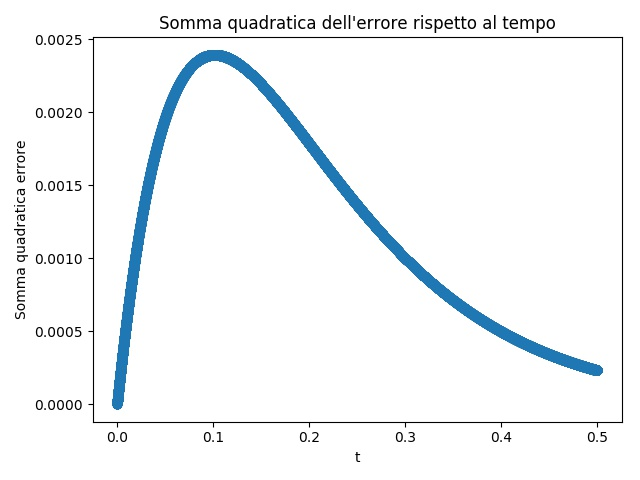
\includegraphics[width=0.4\textwidth]{img/het_cn_M21_N100000.jpg}}\\
	\subfloat[][$h = 0.02,\quad k = 5\times10^{-6}$]{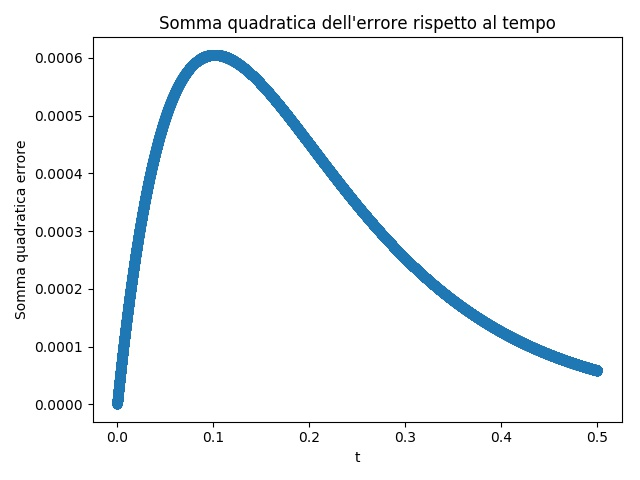
\includegraphics[width=0.4\textwidth]{img/het_cn_M51_N100000.jpg}}
	\subfloat[][$h = 0.006,\quad k = 5\times10^{-6}$]{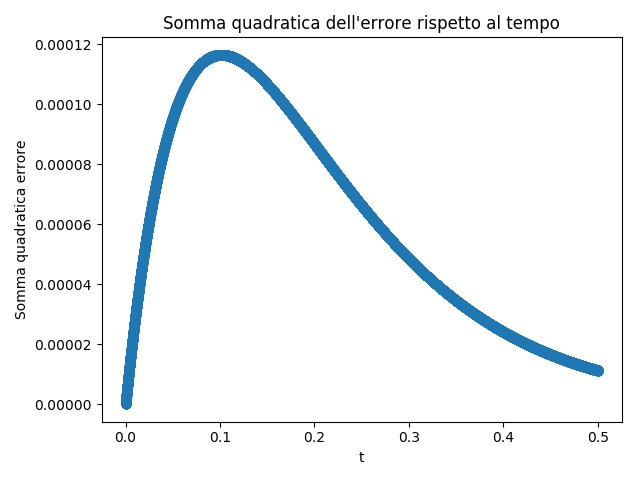
\includegraphics[width=0.4\textwidth]{img/het_cn_M151_N100000.jpg}}
	\caption{Evoluzione della somma quadratica dell'errore nel tempo per il problema della sottosezione \ref{subsec:tronc_imp} a diversi valori di $h$ e $k$}
	\label{fig:troncamento_implicito}
\end{figure}

\begin{figure}
	\centering
	\subfloat[][Andamento quadratico.]{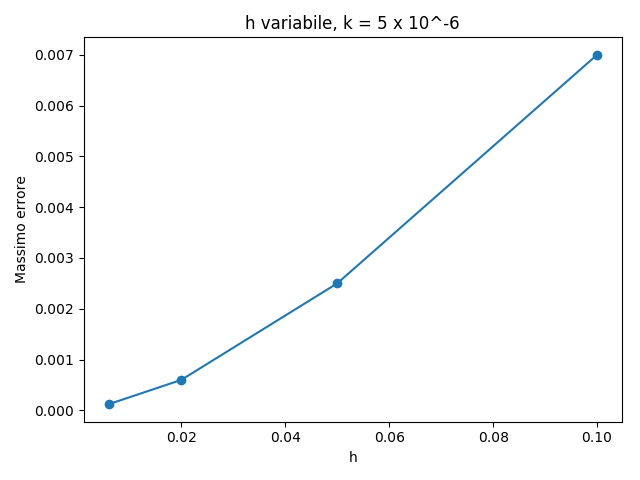
\includegraphics[width=0.45\textwidth]{img/implicit_h.png}}\quad
	\subfloat[][Andamento quadratico.]{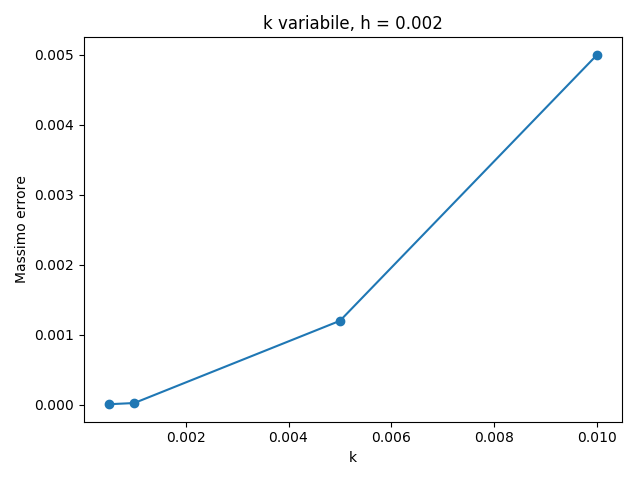
\includegraphics[width=0.45\textwidth]{img/implicit_k.png}}
	\caption{Valori massimi di errore riportati da \ref{fig:troncamento_implicito} su grafico.}
	\label{fig:implicito}
\end{figure}

\begin{figure}
	\centering
	\subfloat[][Integrazione con metodo esplicito, evidenti instabilità presenti.]{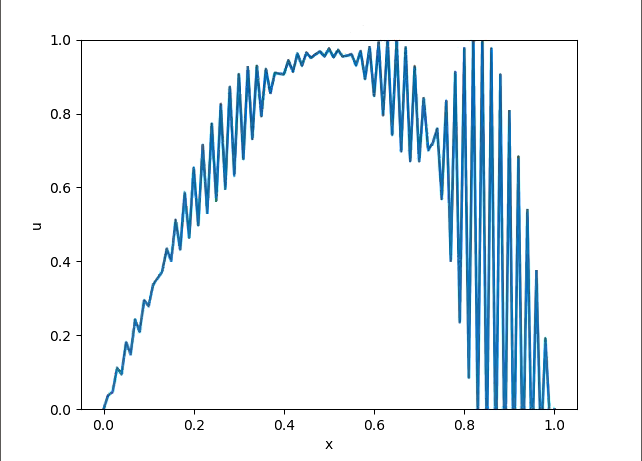
\includegraphics[width=0.45\textwidth]{img/instability47.png}\label{fig:stabilita_esplicito}}\quad
	\subfloat[][Integrazione con metodo di Crank-Nicolson, stabile.]{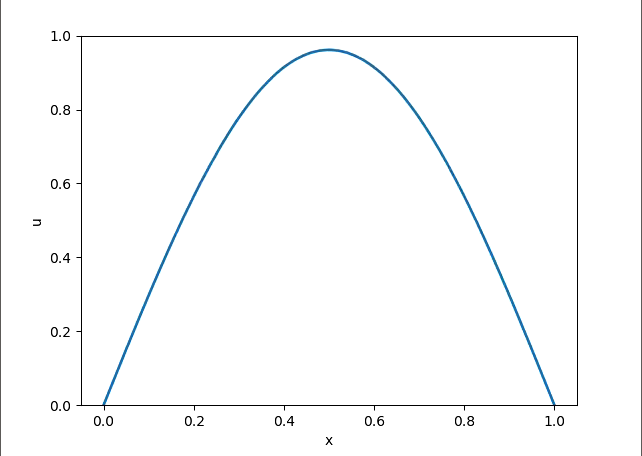
\includegraphics[width=0.45\textwidth]{img/stability47.png}\label{fig:stabilita_implicito}}
	\caption{Integrazione di una equazione del calore con $D=0.1$, $k=0.0008$, $h=0.01$ fino al 47-esimo step temporale.}
	\label{fig:stabilita}
\end{figure}

%%%%%%%%%%%%%%%%%%%%%%%%%%%%%%%%%%%%%%%%%
%%%%%%%%%%%%%%%%%%%%%%%%%%%%%%%%%%%%%%%%%
%%%%%%%%%%%%%%%%%%%%%%%%%%%%%%%%%%%%%%%%%
%%%%%%%%%%%%%%%%%%%%%%%%%%%%%%%%%%%%%%%%%
%%%%%%%%%%%%%%%%%%%%%%%%%%%%%%%%%%%%%%%%%
%%%%%%%%%%%%%%%%%%%%%%%%%%%%%%%%%%%%%%%%%
%%%%%%%%%%%%%%%%%%

\section{Equazione del calore con termine avvettivo e metodo di Crank-Nicolson}

Consideriamo su di una dimensione la seguente equazione differenziale:
\begin{equation}
	\pdv{u}{t} = -A \pdv{u}{x} + B\pdv[2]{u}{x}
\end{equation}
dove consideriamo i termini $A$ e $B$ come valori costanti.

Per convertire ogni termine dell'equazione in forma di differenziale finito scriviamo:
\begin{align}
	\pdv{u}{t} &\Rightarrow \frac{u_m^{n+1}-u_m^n}{k}\\
	\pdv[2]{u}{x} &\Rightarrow \frac{(u_{m+1}^{n+1}-2u_m^{n+1}+u_{m-1}^{n+1}) +(u_{m+1}^{n}-2u_m^{n}+u_{m-1}^{n})}{2(h)^2}\\
	\pdv{u}{x} &\Rightarrow \frac{(u_{m+1}^{n+1}-u_{m-1}^{n+1})+(u_{m+1}^n -u_{m-1}^n)}{4(h)}
\end{align}
definendo poi due costanti per semplificare i conti
\begin{equation}
	\alpha = \frac{Ak}{4(h)}, \quad \beta = \frac{Bk}{2 h^2}
\end{equation}
otteniamo
\begin{multline}
	(\alpha - \beta)(u_{m+1}^{n+1}) + (1 + 2\beta)(u_m^{n+1}) + (-\alpha -\beta)(u_{m-1}^{n+1}) \\= (-\alpha + \beta)(u_{m+1}^n) +(1 -2\beta)(u_m^n) + (\alpha + \beta)(u_{m-1}^n)
\end{multline}
con a sinistra dell'uguale i termini non noti ed a destra dell'uguale i termini noti. È evidente come il problema può venir posto in forma vettoriale
\begin{equation}
	\left(L\right)\vb{u}^{n+1} = \left(R\right)\vb{u}^n + \vb{b},
\end{equation}
dove
\begin{align}
	L &= \mqty*(1+2\beta & \alpha - \beta & 0 & \cdot & \cdot & 0 \\ -\alpha -\beta & 1+2\beta & \alpha-\beta & 0 & \cdot & 0 \\ \cdot & \cdot & \cdot & \cdot & \cdot & \cdot \\ 0 & \cdot & 0 & -\alpha -\beta & 1+2\beta & \alpha-\beta \\ 0 & \cdot & \cdot & 0 & -\alpha-\beta & 1+2\beta);\\
	R &= \mqty*(1-2\beta & -\alpha + \beta & 0 & \cdot & \cdot & 0 \\ \alpha +\beta & 1-2\beta & -\alpha+\beta & 0 & \cdot & 0 \\ \cdot & \cdot & \cdot & \cdot & \cdot & \cdot \\ 0 & \cdot & 0 & \alpha +\beta & 1-2\beta & -\alpha+\beta \\ 0 & \cdot & \cdot & 0 & \alpha+\beta & 1-2\beta);\\
	\vb{b} &= \mqty*((\alpha + \beta)(u_0^n + u_0^{n+1}) \\ 0 \\ \cdot \\ 0 \\ (-\alpha + \beta)(u_M^n + u_M^{n+1})) \equiv \frac{r}{2}\mqty*((\alpha + \beta)(g_0(t_n) + g_0(t_{n+1})) \\ 0 \\ \cdot \\ 0 \\ (-\alpha + \beta)(g_M(t_n) + g_M(t_{n+1}))).
\end{align}
Notiamo poi subito che le matrici $L$ ed $R$ possono essere rispettivamente scritte in forma $(I-A)$ e $(I+A)$ dove $A$ è definita come
\begin{equation}
	A = \mqty*(-2\beta & -\alpha + \beta & 0 & \cdot & \cdot & 0 \\ \alpha +\beta & -2\beta & -\alpha+\beta & 0 & \cdot & 0 \\ \cdot & \cdot & \cdot & \cdot & \cdot & \cdot \\ 0 & \cdot & 0 & \alpha +\beta & -2\beta & -\alpha+\beta \\ 0 & \cdot & \cdot & 0 & \alpha+\beta & -2\beta). 
\end{equation}
Ottenendo quindi
\begin{equation}
	\left(I-A\right)\vb{u}^{n+1} = \left(I+A\right)\vb{u}^n + \vb{b}
\end{equation}

Volendo invece usare la notazione usata nella sezione precedente , utile per le analisi dell'errore di troncamento:
\begin{align}
	\frac{1}{2h}\delta_x u_m &\equiv \frac{u_{m+1}-u_{m-1}}{2h}\\
	\frac{1}{h^2}\delta_x^2 u_m &\equiv \frac{u_{m+1}-2u_m+u_{m-1}}{h^2}\\
	\frac{1}{k}\delta_t u^n &\equiv \frac{u^{n+1}-u^n}{k}
\end{align}
abbiamo la forma (ponendo per semplicità $A=B=1$)
\begin{equation}
	\frac{1}{k}\delta_t u_m^n = \frac{1}{2}\left[\frac{\delta_x^2}{h^2}u_m^n + \frac{\delta_x^2}{h^2}u_m^{n+1} + \frac{\delta_x}{2h}u_m^n + \frac{\delta_x}{2h}u_m^{n+1} \right].
\end{equation}

\subsection{Errore di troncamento}

Facendo riferimento ai risultati ottenuti nella Sottosezione \ref{sec:troncamento}, otteniamo l'ulteriore risultato:
\begin{equation}
	\frac{1}{4h^2}(\delta_x u_m^n + \delta_x u_m^{n+1}) = \bar{u}_{m,x} + O(k^2 + h^2)
\end{equation}
che ci porta a scrivere (si considera per semplicità $A=B=1$)
\begin{multline}
 	\frac{1}{k} \delta_t u_m^n - \frac{1}{2h^2}(\delta_x^2 u_m^n + \delta_x^2 u_m^{n+1}) - \frac{1}{4h}(\delta_x u_m^n + \delta_x u_m^{n+1}) \\= \bar{u}_{m,t} - \bar{u}_{m,xx} -\bar{u}_{m,x} + O(k^2, h^2)
\end{multline} 
che conferma l'errore di troncamento $O(k^2, h^2)$.

\subsection{Analisi di stabilità della matrice}

Avendo posto le matrici in forma più o meno analoga al caso tratato nella Sezione \ref{sec:stabilita_matrice}, possiamo ricondurci al caso di studio in cui poniamo $\vb{b} = 0$ e poniamo l'intero schema nella forma
\begin{equation}
	\vb{u}^{n+1} = \mathcal{M}\vb{u}^n
\end{equation}
per quindi studiare la matrice $\mathcal{M}$ che, in questo contesto, ha forma
\begin{equation}
	\mathcal{M} = (I-A)^{-1}(I+A)
\end{equation}
e possiamo quindi approfittare della forma tridiagonale della matrice $A$ per fare una analisi semplice degli autovalori di $\mathcal{M}$ esattamente come nel caso precedente. Detti $\lambda_j$ gli autovalori della matrice $A$, abbiamo che i corrispondenti autovalori di $\mathcal{M}$ possono essere scritti nella forma:
\begin{equation}
	\frac{1+\lambda_j}{1-\lambda_j},
\end{equation}
sfruttando poi il lemma \ref{lem:tridiagonale} abbiamo che
\begin{align}
	\lambda_j &= -2\beta + 2\sqrt{-\alpha^2 +\beta^2}\cos{\frac{\pi j}{M}}\\
	&= -\frac{Bk}{h^2} +2\sqrt{-\frac{A^2 k^2}{16 h^2} + \frac{B^2 k^2}{4 h^4}}\cos{\phi_j}\\
	&= -\frac{Bk}{h^2} +\frac{k}{h^2}\sqrt{-\frac{A^2 h^2}{4}+B^2}\cos{\phi_j}
\end{align}
dove $\phi_j = \pi j/M$. A questo punto si ha che per avere garantita la stabilità si deve avere
\begin{equation}
	\abs{\frac{h^2 - k (+ B - \sqrt{-\frac{A^2 h^2}{4}+B^2} \cos{\phi_j})}{h^2 + k (+ B - \sqrt{-\frac{A^2 h^2}{4}+B^2} \cos{\phi_j})}} \leq 1
\end{equation}
dove possiamo distinguere due situazioni: 
\begin{itemize}
	\item L'argomento sotto le radici quadrate è positivo. Avendo quindi intuitivamente che $B > \sqrt{B^2 - A^2h^2/4}$, si ha che l'argomento dentro le parentesi tonde è sempre di segno positivo e, di conseguenza, il modulo intero è sempre minore di 1.
	\item L'argomento sotto le radici quadrate è negativo. Questo implica che abbiamo a che fare con un valore immaginario e, di conseguenza, autovalori complessi. Abbiamo quindi da la disequazione
	\begin{multline}
		\abs{h^2 - kB + ik\sqrt{\abs{-\frac{A^2 h^2}{4}+B^2}} \cos{\phi_j}} \\\leq \abs{h^2 + kB - ik\sqrt{\abs{-\frac{A^2 h^2}{4}+B^2}} \cos{\phi_j}},
	\end{multline}
	che è equivalente a scrivere
	\begin{multline}
		\abs{h^2 - kB }+\abs{+ ik\sqrt{\abs{-\frac{A^2 h^2}{4}+B^2}} \cos{\phi_j}} \\\leq \abs{h^2 + kB }+\abs{- ik\sqrt{\abs{-\frac{A^2 h^2}{4}+B^2}} \cos{\phi_j}},
	\end{multline}
	che risulta sempre valida.
\end{itemize}
Abbiamo pertanto che, anche in questo caso, lo schema risulta incondizionatamente stabile.

\subsection{Risultati numerici}

Come problema di prova, consideriamo una equazione semplice del calore con termine avvettivo nell'intervallo $x\in[0,1]$ con condizioni al contorno periodiche (si veda Appendice \ref{app:boundaries} su come trattare questa tipologia di condizioni al contorno):
\begin{align}
	\pdv{u}{t} &= -A\pdv{u}{x} + B\pdv[2]{u}{x},\quad\quad 0\leq x\leq 1\\
	u(0,t) &= u(1,t)
\end{align}
E, come condizione iniziale (Appendice \ref{app:soluzione_fokker_planck}),
\begin{equation}
	u(x,0) = \frac{1}{2\sqrt{\pi B t_0}}\exp\left[-\frac{((x+0.5)+(-A)t_0)^2}{4Bt_0}\right].
\end{equation}
Come valori numerici si impostano\\
\begin{center}
	\begin{tabular}{cS}
	 \toprule
	 Costante & {Valore}\\
	 \midrule
	 $A$ & 10.\\
	 $B$ & 0.5\\
	 $t_0$ & 0.001\\
	 $t_{\text{target}}$ & 0.5\\
	 $h$ & 0.005\\
	 $k$ & 0.000005\\
	 \bottomrule 
	\end{tabular}
\end{center}
La somma quadratica degli errori è riportata in figura \ref{fig:foc_cn_errore} e viene comparata con i valori assunti dalla soluzione analitica in figura \ref{fig:foc_cn_relativo}. È possibile inoltre visualizzare l'integrazione numerica su di un supporto video.

\begin{figure}
	\centering
	\subfloat[][Somma quadratica dell'errore.]{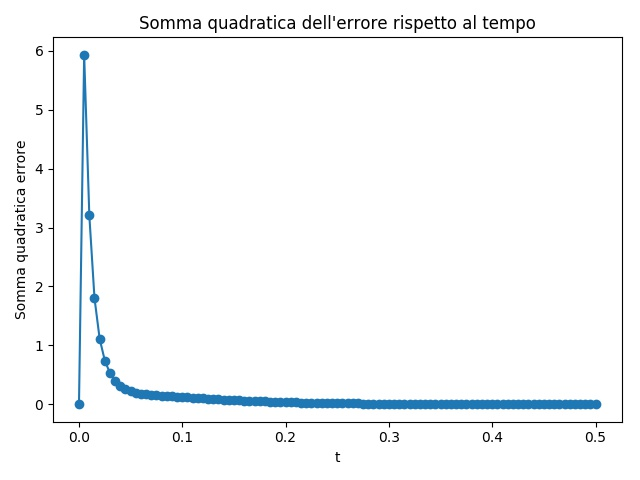
\includegraphics[width=0.4\textwidth]{img/fok_cn_M101_N100.jpg}\label{fig:foc_cn_errore}}\quad
	\subfloat[][Rapporto in percentuale tra la Somma quadratica dell'errore e la somma dei valori della soluzione analitica.]{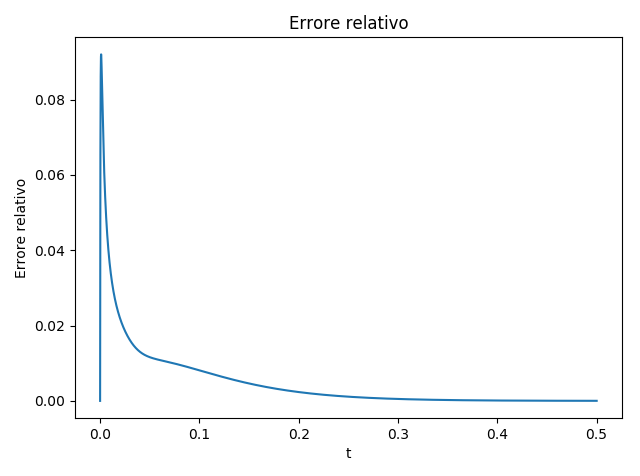
\includegraphics[width=0.4\textwidth]{img/errore_relativo.png}\label{fig:foc_cn_relativo}}
	\caption{Errore per integrazione di equazione di Fokker Planck con Crank-Nicolson.}
	\label{fig:implicito}
\end{figure}

%%%%%%%%%%%%%%%%%%%%%%%%%%%%%%%%%%%%%%%%%%%%%%%
%%%%%%%%%%%%%%%%%%%%%%%%%%%%%%%%%%%%%%%%%%%%%%%
%%%%%%%%%%%%%%%%%%%%%%%%%%%%%%%%%%%%%%%%%%%%%%%
%%%%%%%%%%%%%%%%%%%%%%%%%%%%%%%%%%%%%%%%%%%%%%%
%%%%%%%%%%%%%%%%%%%%%%%%%%%%%%%%%%%%%%%%%%%%%%%

\appendix

\section{Soluzione esatta per equazione del calore}
\label{app:soluzione_esatta}

La soluzione generale per una equazione nella forma
\begin{equation}
	\pdv{u}{t} = D \pdv[2]{u}{x}
\end{equation}
in un intervallo $0\leq x \leq L$ con condizioni al contorno nulle è data da
\begin{equation}
	u(x,t) = \sum_{n=1}^\infty b_n \sin\left(\frac{n\pi x}{L}\right) \exp\left(-\frac{D n^2 \pi^2 t}{L^2}\right)
\end{equation}
dove i coefficienti $b_n$ sono dati da
\begin{equation}
	b_n = \frac{2}{L}\int_0^L u_0(x)\sin\left(\frac{n\pi x}{L}\right)\,dx
\end{equation}
dove $u_0(x)$ è la condizione iniziale.

\paragraph{Esempio: $u_0(x) = \sin(\pi x / L)$}.
Si ha che
\begin{equation}
	b_n = \frac{2}{L}\int_0^L \sin(\pi x / L)\sin\left(\frac{n\pi x}{L}\right)\,dx
\end{equation}
che risulta però avere valore non nullo solo nel caso in cui $n=1$, in cui assume il valore $1$. Pertanto si ha che la soluzione esatta dell'equazione è
\begin{equation}
	u(x,t) = \sin\left(\frac{\pi x}{L}\right)\exp\left(-\alpha \pi^2 t / L^2 \right).
\end{equation}

\section{Soluzione esatta per equazione del calore con termine avvettivo}
\label{app:soluzione_fokker_planck}
Come soluzione analitica per l'equazione differenziale
\begin{equation}
	\pdv{u}{t} = -A\pdv{u}{x} + B\pdv[2]{u}{x}
\end{equation}
si considera la soluzione fondamentale
\begin{equation}
	u(x,t) = \frac{1}{2\sqrt{\pi B t}}\exp\left[-\frac{(x+(-A)t)^2}{4Bt}\right]
\end{equation}
e, per trattare una situazione semplice da gestire a livello numerico, si considera come condizione iniziale l'evoluto di
\begin{equation}
	u(x,0) = \delta(x-0.5)
\end{equation}
per un tempo piccolo $t_0$.

\section{Discretizzazione di equazioni paraboliche a derivate parziali con coefficienti variabili per Crank-Nicolson}

Per poter trattare una equazione nella forma
\begin{equation}
	u_t = a(x,t)u_{xx} + b(x,t)u_{x} + c(x,t)u
\end{equation}
ci interessa formulare una discretizzazione che mantenga la precisione dell'ordine di $O(k^2+h^2)$. Sfruttando il fatto che
\begin{equation}
	\frac{f(x+h)-f(x-h)}{2h} = f'(x)+O(h^2),
\end{equation}
o, equivalentemente
\begin{equation}
	\frac{f(x+h)-f(x-h)}{h} = f'\left(x + \frac{h}{2}\right)+O(h^2),
\end{equation}
dove $f(x)$ è una funzione sufficientemente regolare, possiamo scrivere che
\begin{align}
	u_t &\to \frac{1}{k}\delta_t u_m^n\\
	a(x,t)u_{xx} &\to \frac{1}{2h^2}(a_m^n \delta^2_x u_m^n + a_m^{n+1} \delta_x^2 u_m^{n+1})\\
	b(x,t)u_x &\to \frac{1}{4h} (b_m^n (u_{m+1}^n - u_{m-1}^n) + b_m^{n+1}(u_{m+1}^{n+1}-u_{m-1}^{n+1}))\\
	c(x,t)u &\to \frac{1}{2}(c_m^nu_m^n + c_m^{n+1}u_m^{n+1}). 
\end{align}

Spesso si ha a che fare con equazioni a derivate parziali nella forma
\begin{equation}
	\gamma(x,t)\pdv{u}{t} = \pdv{}{x}\left(\alpha(x,t) \pdv{u}{x}\right) + \beta(x,t)u
\end{equation}
per quanto possa essere espansa e ricondotta a forme più semplici, è possibile discretizzarla direttamente nella forma:
\begin{align}
	\gamma(x,t)u_t &\to \frac{1}{2}(\gamma_m^n+\gamma_m^{n+1})\frac{1}{k}\delta_t u_m^n, \quad \text{oppure} \quad \gamma_m^{n+\frac{1}{2}}\frac{1}{k}\delta_t u_m^n \\
	(\alpha(x,t)u_x)_x &\to \frac{1}{2h}\left(\alpha_{m+\frac{1}{2}}^n \frac{\delta_x u_m^n}{h} - \alpha_{m-\frac{1}{2}}^n \frac{\delta_x u_{m-1}^n}{h}\right) + \frac{1}{2h}\left(\alpha_{m+\frac{1}{2}}^{n+1} \frac{\delta_x u_m^{n+1}}{h} - \alpha_{m-\frac{1}{2}}^{n+1} \frac{\delta_x u_{m-1}^{n+1}}{h}\right) \\
	\beta(x,t)u &\to \frac{1}{2}(\beta_m^n u_m^n + \beta_m^{n+1}u_m^{n+1}).
\end{align}

%%%%%%%%%%%%%%%%%%%%%%%%%%%%%%
%%%%%%%%%%%%%%%%%%%%%%%%%%%%%%
%%%%%%%%%%%%%%%%%%%%%%%%%%%%%%

\section{Trattazione di diverse tipologie di condizioni al contorno in Crank-Nicolson}
\label{app:boundaries}
\paragraph{Condizioni al contorno periodiche.}
Qualora si vogliano imporre condizioni al contorno periodiche, queste si esprimono nella forma $u_0^n = u_M^n$, che può quindi essere implementata direttamente all'interno della matrice $A$ del metodo.

Se per esempio volessimo trattare il problema dell'equazione del calore in Sezione \ref{sec:2} con condizioni al contorno periodiche, avremmo che la matrice $A$ passerebbe dalla forma in equazione \eqref{eq:A_calore_CN} alla forma:
\begin{equation}
	A = \mqty*(-2 & 1 & 0 & \cdot & 0 & 1 \\ 1 & -2 & 1 & 0 & \cdot & 0 \\ \cdot & \cdot & \cdot & \cdot & \cdot & \cdot \\ 0 & \cdot & 0 & 1 & -2 & 1 \\ 1 & 0 & \cdot & 0 & 1 & -2)
\end{equation}
e non si avrebbe più il vettore $\vb{b}$ nell'espressione. Questo inevitabilmente porta alla rottura della struttura tridiagonale della matrice e richiede quindi un approccio leggermente diverso nell'analisi e nella risoluzione.

\paragraph{Condizioni al contorno riflettenti.}
Imporre una condizione al contorno riflettente (per esempio su $x=0$) equivale ad imporre che
\begin{equation}
	\pdv{}{x} u_0^n = 0
\end{equation}
sfruttando quindi la discretizzazione al secondo ordine $O(h^2)$ possiamo scrivere
\begin{equation}
	\pdv{}{x}u_0^n \approx \frac{-3u_0^n + 4_h^n - u_{2h}^n}{2h}
\end{equation}
possiamo quindi imporre la condizione all'approssimazione e moltiplicare entrambi i lati per $2h$, ottenendo
\begin{equation}
	-3u_0^n + 4_h^n - u_{2h}^n = 0
\end{equation}
che, risolta per $u_0^n$ ritorna:
\begin{equation}
	u_0^n = \frac{4}{3}u_{h}^n - \frac{1}{3}u_{2h}^n
\end{equation}
che può essere quindi implementata dentro la matrice $A$ che descrive gli step del metodo.

\end{document}

